\documentclass[12pt, a4paper]{article}

% ── Packages ──────────────────────────────────────────────────────────────────
\usepackage[a4paper, margin=2.5cm]{geometry}
\usepackage{graphicx}
\usepackage{float}
\usepackage{amsmath}
\usepackage{amssymb}
\usepackage{xcolor}
\usepackage{mdframed}
\usepackage{parskip}
\usepackage{enumitem}
\usepackage{titlesec}
\usepackage{booktabs}
\usepackage{hyperref}
\usepackage[T1]{fontenc}
\usepackage{tikz}
\usepackage{listings}
\usetikzlibrary{arrows.meta}

% ── Graphics path ─────────────────────────────────────────────────────────────
\graphicspath{{../../Images_for_latex/Lecture_4/}}

% ── Colours ───────────────────────────────────────────────────────────────────
\definecolor{keyblue}{RGB}{30, 80, 160}
\definecolor{keybluebg}{RGB}{220, 235, 255}
\definecolor{noteorange}{RGB}{200, 100, 0}
\definecolor{noteorangebg}{RGB}{255, 240, 215}
\definecolor{warnred}{RGB}{180, 30, 30}
\definecolor{warnredbg}{RGB}{255, 220, 220}
\definecolor{defgreen}{RGB}{20, 110, 50}
\definecolor{defgreenbg}{RGB}{215, 245, 225}
\definecolor{headernavy}{RGB}{25, 35, 90}

% ── Box environments ──────────────────────────────────────────────────────────
\newmdenv[linecolor=keyblue,backgroundcolor=keybluebg,linewidth=1.5pt,
  leftline=true,rightline=false,topline=false,bottomline=false,
  innerleftmargin=10pt,innerrightmargin=8pt,
  innertopmargin=6pt,innerbottommargin=6pt,
  skipabove=8pt,skipbelow=8pt]{keybox}

\newmdenv[linecolor=noteorange,backgroundcolor=noteorangebg,linewidth=1.5pt,
  leftline=true,rightline=false,topline=false,bottomline=false,
  innerleftmargin=10pt,innerrightmargin=8pt,
  innertopmargin=6pt,innerbottommargin=6pt,
  skipabove=8pt,skipbelow=8pt]{notebox}

\newmdenv[linecolor=warnred,backgroundcolor=warnredbg,linewidth=1.5pt,
  leftline=true,rightline=false,topline=false,bottomline=false,
  innerleftmargin=10pt,innerrightmargin=8pt,
  innertopmargin=6pt,innerbottommargin=6pt,
  skipabove=8pt,skipbelow=8pt]{warnbox}

\newmdenv[linecolor=defgreen,backgroundcolor=defgreenbg,linewidth=1.5pt,
  leftline=true,rightline=false,topline=false,bottomline=false,
  innerleftmargin=10pt,innerrightmargin=8pt,
  innertopmargin=6pt,innerbottommargin=6pt,
  skipabove=8pt,skipbelow=8pt]{defbox}

% ── Section formatting ────────────────────────────────────────────────────────
\titleformat{\section}[block]{\large\bfseries\color{headernavy}}{}{0pt}{}
  [\vspace{2pt}\rule{\linewidth}{0.8pt}\vspace{4pt}]
\titleformat{\subsection}[block]{\normalsize\bfseries\color{keyblue}}{}{0pt}{}

% ── Document ──────────────────────────────────────────────────────────────────
\begin{document}

\section*{Lecture 4 --- UKF vs Linear KF}
\vspace{-0.5cm}
\subsection*{Exercise 1: Scalar Nonlinear System}
\vspace{-0.2cm}
We are given a scalar system, nonlinear in \textbf{both} transition $f$ and measurement $h$.
A linear approximation is obtained by setting $\varphi_f = \varphi_h = 0$ and $\sin(x) \approx x$:
\[
\begin{array}{rl@{\qquad\qquad}rl}
  \multicolumn{2}{c}{\textbf{Nonlinear}} & \multicolumn{2}{c}{\textbf{Linear approximation}} \\[6pt]
  x_k &= a\sin(x_{k-1} + \varphi_f) + bu_{k-1} + w_{k-1}
  & x_k &= ax_{k-1} + bu_{k-1} + w_{k-1} \\[4pt]
  z_k &= \sin(cx_k + \varphi_h) + v_k
  & z_k &= cx_k + v_k \\[8pt]
  \multicolumn{4}{c}{\textbf{For both}} \\[4pt]
  \multicolumn{4}{c}{w \in \text{NID}(0,Q) \text{ Process noise}, \quad v \in \text{NID}(0,R) \text{ Measurement noise}, \quad x_0 \in \mathcal{N}(\hat{x}_0,\,P_0) \text{Initial guess}}
\end{array}
\]
The standard linear KF is applied to the linear system, while the UKF is applied
directly to the nonlinear system --- no linearisation needed.
\vspace{-0.4cm}
\subsection*{Why the linear KF cannot handle nonlinear systems}
\vspace{-0.2cm}
The linear KF operates entirely through matrix multiplication:
\[
  x_{k+1} = \boldsymbol{\Phi}x_k + Lu_k, \qquad z_k = Hx_k
\]
which can only scale and rotate --- never bend or curve.

The deeper problem is \textbf{covariance propagation}: the KF assumes uncertainty
remains Gaussian after passing through $f$ and $h$, but a nonlinear function
distorts a Gaussian into a non-Gaussian shape --- the mean and covariance alone
no longer fully describe it.
Forcing a nonlinear $f$ or $h$ into $\boldsymbol{\Phi}$ and $H$ introduces
linearisation error that grows as the state moves away from the operating point,
and the propagated covariance increasingly misrepresents the true uncertainty shape.
\vspace{-0.4cm}
\subsection*{UKF --- handling nonlinearity without linearisation}
\vspace{-0.2cm}
The state estimate (mean) can still be pushed directly through $f$ and $h$,
but the covariance no longer describes the correct shape of the uncertainty
after a nonlinear transformation --- a Gaussian mapped through a nonlinearity
becomes skewed or multimodal.
\textbf{Meaning the mean and covariance alone are insufficient to fully characterise it.}

Both \textbf{EKF} and \textbf{UKF} approximate a solution by still
assuming Gaussian uncertainty, but differ in how accurately they propagate
the covariance through the nonlinearity.

We use the UKF here for two reasons:
\begin{itemize}[leftmargin=1.4em]
  \item \textbf{Higher accuracy:} the EKF handles nonlinearity by linearising
        $f$ and $h$ around the current estimate using the \textbf{Jacobian}:
        \[
          F = \frac{\partial f}{\partial x}\bigg|_{\hat{x}_k}, \qquad
          H = \frac{\partial h}{\partial x}\bigg|_{\hat{x}_k}
        \]
        This is a 1st-order approximation --- it captures the local slope but
        ignores curvature (2nd-order effects), so the propagated covariance
        is only approximately correct.
        The UKF instead propagates sigma points directly through $f$ and $h$,
        reconstructing the covariance from the spread of the transformed points
        --- capturing up to 2nd-order effects without any derivatives.

  \item \textbf{No Jacobian required:} computing $F$ and $H$ analytically is
        tedious and error-prone for complex functions. The UKF treats $f$ and
        $h$ as black-box functions --- only evaluations are needed, not derivatives.
\end{itemize}

\begin{notebox}
  \textbf{Example of this skewed thing}
\begin{figure}[H]
\centering
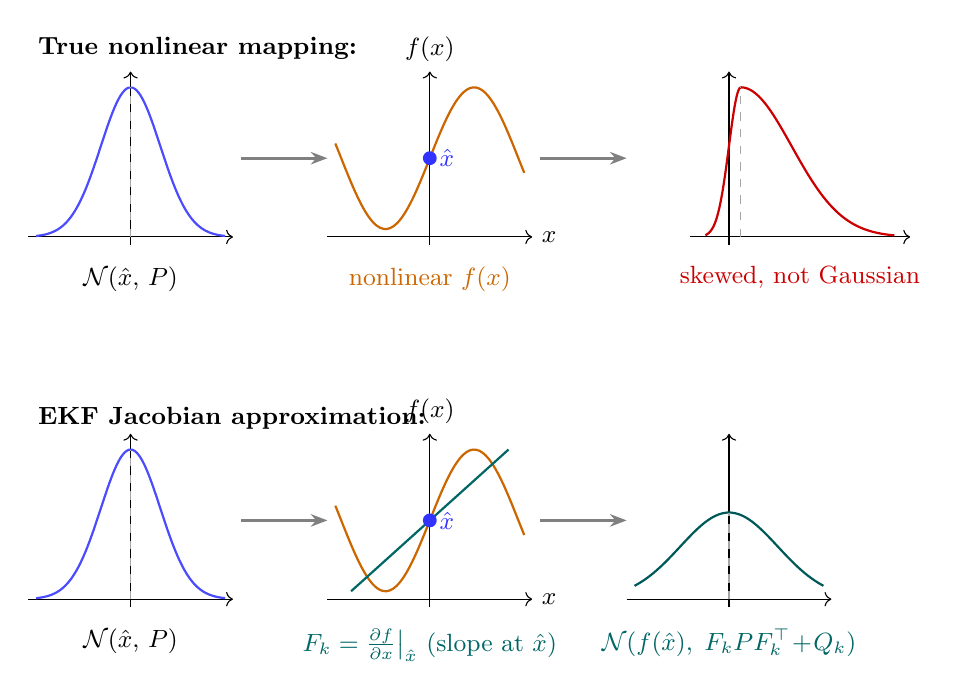
\begin{tikzpicture}[
    arr/.style={-{Stealth[length=6pt]}, very thick},
    lbl/.style={font=\small}
  ]

  % ══ ROW 1: true nonlinear ═════════════════════════════════════════════════
  \node[font=\bfseries\small, anchor=west] at (-1.3, 6.2)
    {True nonlinear mapping:};

  % LEFT: input Gaussian
  \begin{scope}[yshift=3.8cm]
    \draw[->] (-1.3,0) -- (1.3,0);
    \draw[->] (0,-0.1) -- (0,2.1);
    \draw[blue!70, thick, domain=-1.2:1.2, smooth, samples=50]
      plot (\x, {1.9*exp(-3.5*\x*\x)});
    \draw[dashed, gray!70] (0,0) -- (0,1.9);
    \node[lbl, below] at (0,-0.25) {$\mathcal{N}(\hat{x},\,P)$};
  \end{scope}

  % MIDDLE: nonlinear function f(x) = sin(x), no tangent
  \begin{scope}[xshift=3.8cm, yshift=3.8cm]
    \draw[->] (-1.3,0) -- (1.3,0) node[right, lbl]{$x$};
    \draw[->] (0,-0.1) -- (0,2.1) node[above, lbl]{$f(x)$};
    \draw[orange!80!black, thick, domain=-1.2:1.2, smooth, samples=60]
      plot (\x, {1.0 + 0.9*sin(160*\x)});
    \fill[blue!80] (0, 1.0) circle (2.5pt)
      node[right, lbl]{$\hat{x}$};
    \node[lbl, below, orange!80!black] at (0,-0.25) {nonlinear $f(x)$};
  \end{scope}

  % arrow left to middle
  \draw[arr, gray] (1.4, 4.8) -- (2.5, 4.8);

  % RIGHT: skewed output
  \begin{scope}[xshift=7.6cm, yshift=3.8cm]
    \draw[->] (-0.5,0) -- (2.3,0);
    \draw[->] (0,-0.1) -- (0,2.1);
    \draw[red!80!black, thick, domain=-0.3:2.1, smooth, samples=100]
      plot (\x, {ifthenelse(\x < 0.15,
                  1.9*exp(-22*(\x-0.15)*(\x-0.15)),
                  1.9*exp(-1.2*(\x-0.15)*(\x-0.15)))});
    \draw[dashed, gray!70] (0.15,0) -- (0.15,1.9);
    \node[lbl, below, red!80!black] at (0.9,-0.25) {skewed, not Gaussian};
  \end{scope}

  % arrow middle to right
  \draw[arr, gray] (5.2, 4.8) -- (6.3, 4.8);

  % ══ ROW 2: EKF Jacobian ═══════════════════════════════════════════════════
  \node[font=\bfseries\small, anchor=west] at (-1.3, 1.5)
    {EKF Jacobian approximation:};

  % LEFT: same input Gaussian
  \begin{scope}[yshift=-0.8cm]
    \draw[->] (-1.3,0) -- (1.3,0);
    \draw[->] (0,-0.1) -- (0,2.1);
    \draw[blue!70, thick, domain=-1.2:1.2, smooth, samples=50]
      plot (\x, {1.9*exp(-3.5*\x*\x)});
    \draw[dashed, gray!70] (0,0) -- (0,1.9);
    \node[lbl, below] at (0,-0.25) {$\mathcal{N}(\hat{x},\,P)$};
  \end{scope}

  % MIDDLE: same nonlinear function WITH tangent line at x_hat
  \begin{scope}[xshift=3.8cm, yshift=-0.8cm]
    \draw[->] (-1.3,0) -- (1.3,0) node[right, lbl]{$x$};
    \draw[->] (0,-0.1) -- (0,2.1) node[above, lbl]{$f(x)$};
    % nonlinear curve
    \draw[orange!80!black, thick, domain=-1.2:1.2, smooth, samples=60]
      plot (\x, {1.0 + 0.9*sin(160*\x)});
    % tangent line at x_hat=0, slope = F_k = 0.9*cos(0) = 0.9
    \draw[teal!80!black, thick, domain=-1.0:1.0]
      plot (\x, {1.0 + 0.9*\x});
    % dot at mean
    \fill[blue!80] (0, 1.0) circle (2.5pt)
      node[right, lbl]{$\hat{x}$};
    \node[lbl, below, teal!80!black] at (0,-0.25)
      {$F_k = \frac{\partial f}{\partial x}\big|_{\hat{x}}$ (slope at $\hat{x}$)};
  \end{scope}

  % arrow left to middle
  \draw[arr, gray] (1.4, 0.2) -- (2.5, 0.2);

  % RIGHT: Gaussian output (wider, still symmetric)
  \begin{scope}[xshift=7.6cm, yshift=-0.8cm]
    \draw[->] (-1.3,0) -- (1.3,0);
    \draw[->] (0,-0.1) -- (0,2.1);
    \draw[teal!70!black, thick, domain=-1.2:1.2, smooth, samples=50]
      plot (\x, {1.1*exp(-1.3*\x*\x)});
    \draw[dashed, gray!70] (0,0) -- (0,1.1);
    \node[lbl, below, teal!80!black, align=center] at (0,-0.25)
      {$\mathcal{N}(f(\hat{x}),\;F_kPF_k^\top\!+\!Q_k)$};
  \end{scope}

  % arrow middle to right
  \draw[arr, gray] (5.2, 0.2) -- (6.3, 0.2);

\end{tikzpicture}
\caption{Top row: the true nonlinear $f$ warps the Gaussian into a skewed
         non-Gaussian --- no simple covariance formula exists.
         Bottom row: the EKF draws a tangent line on $f$ at $\hat{x}$,
         giving slope $F_k$ (the Jacobian). The uncertainty $P$ is then
         propagated through that slope as $F_kPF_k^\top + Q_k$,
         keeping the output Gaussian --- accurate near $\hat{x}$,
         increasingly wrong further away.}
\end{figure}
\end{notebox}


\clearpage
\section*{UKF - Step by Step}
\vspace{-0.3cm}
The UKF can be seen as a smarter Monte Carlo approach --- instead of randomly
sampling many points, we place $2n+1$ sigma points at carefully chosen locations
that capture the current state estimation uncertainty $P$ (how uncertain we are
about where the true state actually is, given all measurements seen so far).

Each sigma point is passed through the nonlinear $f$ and $h$ directly, and
weighted contributions from all points reconstruct both the predicted mean
(state estimate) and the predicted covariance. The weights control how much
each point influences both --- points closer to the mean carrying more weight
than those at the edges.
\vspace{-0.4cm}
\subsection*{Step 1 Parameters: default values ()$\alpha=1$,
$\kappa=2$, $\beta=0$ give $\lambda = 2$)}
\vspace{-0.2cm}
\[
  \lambda = \alpha^2(n+\kappa) - n, \qquad
  k = \sqrt{n+\lambda}, \qquad
  n = \dim(x)
\]
These points can be disrbuted differnt depending on set parametars
\begin{itemize}
  \item $\lambda$ is a scaling parameter controlling how far the sigma points
are spread from the mean.
  \item $k$ is the actual distance multiplier used
  when placing them.
\end{itemize}
\begin{notebox}
  With the default values and $n=2$ states: $\lambda = 1^2(2+2)-2 = 2$, $k = \sqrt{2+2} = 2$.
\end{notebox}
\vspace{-0.3cm}
The larger $n$ is, the further out the points are placed to
cover the wider spread of a higher-dimensional Gaussian.
\vspace{-0.4cm}
\subsection*{Step 2 --- Sigma points (eigendecomposition)}
\vspace{-0.2cm}
The scaled covariance $(n+\lambda)P$ is decomposed via \texttt{np.linalg.eigh}:
\[
  (n+\lambda)P = V L V^\top, \qquad
  S = V\sqrt{L} 
\]
where:
\begin{itemize}[leftmargin=1.4em]
  \item $L = \text{diag}(l_1,\ldots,l_n)$ --- eigenvalues, variance magnitude in each direction
  \item $V = [u_1,\ldots,u_n]$ --- eigenvectors, which directions the uncertainty points in
  \item $S = V\sqrt{\Lambda}$ --- matrix square root of $(n+\lambda)P$,
        each column $S_{:,i} = u_i\sqrt{l_i}$ gives the offset direction and magnitude
\end{itemize}

The $2n+1$ sigma points are placed symmetrically around the mean
(also written as $\mu_x = \hat{x}$, $k = \sqrt{n+\lambda}$ in lecture notation):
\[
  SigmaPT_i = \begin{cases}
    \mu_x            \quad =\hat{x} & i = 0 \quad \text{(center: current mean estimate)}\\
    \mu_x + u_i\sqrt{l_i}  \quad= \hat{x} + S_{:,i}   & 1 \leq i \leq n \quad \text{(pushed positive along } u_i\text{)}\\
    \mu_x- u_{i-n}\sqrt{l_{i-n}} \quad= \hat{x} - S_{:,i-n} & n+1 \leq i \leq 2n \quad \text{(symmetric negative push)}
  \end{cases}
\]
\begin{notebox}
The \texttt{np.maximum(eigvals, 0)} clips any floating-point negative eigenvalues
before the square root --- $P$ should be positive definite but numerical drift
can produce tiny negatives after many steps. Which could break the filter --- the clip prevents this.
\end{notebox}
\clearpage
\subsection*{step 3: Weighting of Mean and Covariance}
Each sigma point is assigned two weights --- one controlling its contribution
to the predicted mean, one to the predicted covariance:
\[
  \underbrace{w_i^m= \begin{cases}
    \dfrac{\lambda}{n+\lambda} & i = 0 \\[6pt]
    \dfrac{1}{2(n+\lambda)}    & 1 \leq i \leq 2n
  \end{cases}}_{\text{weight mean}}
  \qquad
  \underbrace{w_i^c = \begin{cases}
    \dfrac{\lambda}{n+\lambda} + (1 - \alpha^2 + \beta) & i = 0 \\[6pt]
    \dfrac{1}{2(n+\lambda)}    & 1 \leq i \leq 2n
  \end{cases}}_{\text{weight covariance}}
\]
The centre point $\sigma_0 = \hat{x}$ gets a higher weight since it sits
exactly at the mean estimate. The covariance weight $W_0^c$ has the extra
term $(1 - \alpha^2 + \beta)$ to allow fine-tuning of how much the centre
point contributes to the spread --- $\beta = 2$ is optimal for Gaussian
distributions. All weights sum to 1.

\begin{notebox}
  \textbf{Weights are fixed} --- computed once from $\alpha, \kappa, \beta, n$ and
  reused every step. Two sets exist so the centre point's contribution to the
  covariance can be tuned independently via $(1-\alpha^2+\beta)$, without
  affecting the mean weight.

  \textbf{Example} ($n=1, \alpha=1, \lambda=1, \beta=2$):
  \begin{itemize}[leftmargin=1.4em, topsep=2pt]
    \item $\underbrace{W_0^m}_{\text{centre}} = \frac{1}{2} = 0.5$, \quad
          $\underbrace{W_{1,2}^m}_{\text{outer points}} = \frac{1}{4} = 0.25$ \quad
          $\rightarrow$ sum $= 1$ \checkmark
    \item $\underbrace{W_0^c}_{\text{centre}} = 0.5 + \underbrace{(1-1+2)}_{\text{tuning term}} = 2.5$, \quad
          $\underbrace{W_{1,2}^c}_{\text{outer points}} = 0.25$ \quad
          $\rightarrow$ centre weighted more 
  \end{itemize}
\end{notebox}
\vspace{-0.7cm}
\subsection*{Step 4 - Propagate and compute output statistics.}
Each of the $2n+1$ sigma points is pushed through the nonlinear $f$ together
with the known input $u$ --- no Jacobian, no approximation:
\[
  \sigma_i^{\text{pred}} = f(\sigma_i,\, u), \qquad i = 0, 1, \ldots, 2n
\]
where $u$ is identical for all points since it is a known deterministic input ---
only the state uncertainty $\sigma_i$ varies across the points.

We then use the weights to reconstruct the predicted mean and covariance
from the spread of the propagated points:

\textbf{Predicted state mean}

weighted average of where the sigma points land after $f$:
\[
  \hat{x}_{k+1|k} = \sum_{i=0}^{2n} W_i^m\, \sigma_i^{\text{pred}}
\]
\textbf{Predicted state covariance}

weighted sum of how far each propagated sigma point is from the predicted mean, giving the spread of uncertainty after $f$,
plus the irreducible process noise $Q$:
\[
  P_{k+1|k} = Q + \sum_{i=0}^{2n} W_i^c\,
    \underbrace{\bigl(\sigma_i^{\text{pred}} - \hat{x}_{k+1|k}\bigr)
    \bigl(\sigma_i^{\text{pred}} - \hat{x}_{k+1|k}\bigr)^\top}_{\text{outer product: spread of point } i \text{ from mean}}
\]
Because $Q$ adds irreducible process noise each step, and the nonlinear $f$
warps the sigma points unevenly --- the curve is steeper in some places and
flatter in others, so the outer points land at different distances from the
predicted mean $\hat{x}_{k+1|k}$, breaking the symmetry and generally
increasing the spread compared to a linear propagation.

\subsection*{Still Step 4 Just Now on the measurement side}

From the system equation $z_k = h(x_k) + v_k$, it may seem natural to simply
push the predicted state $\hat{x}_{k+1|k}$ through $h$. However
$\hat{x}_{k+1|k}$ is only the \textbf{single weighted mean} --- one point
that discards all uncertainty information.

Instead we push all $2n+1$ propagated sigma points through $h$:
\[
  z_{\text{sig},i} = h(\sigma_i^{\text{pred}}), \qquad i = 0,\ldots,2n
\]
This preserves the full spread of uncertainty through the nonlinear $h$,
following the same logic as Step 4.
\begin{notebox}
the sigma points represent the
distribution of $x_k$, so passing them through $h$ gives the distribution
of $z_k$. Collapsing to $\hat{x}_{k+1|k}$ first and then pushing through
$h$ would lose all covariance information and reduce to a linear-style update.
\end{notebox}

We then use actually these $z_{\text{sig},i}$ to calcualte the weighted measurements.

\textbf{predicted measurement mean}

weighted average of where the sigma points land after $h$ using same wiegth mean as from the \textbf{predicted state mean}:
\[
  \hat{z}_{k+1|k} = \sum_{i=0}^{2n} W_i^m\, z_{\text{sig},i}
\]
\textbf{$S_{zz}$ increases} because we add $R$ on top of the sigma point
spread --- the sensor always adds irreducible noise regardless of how well
the sigma points capture the state uncertainty.


\textbf{Innovation covariance}

Total measurement uncertainty, analogous to $S = HPH^\top + R$ in the linear KF but computed from the spread of
sigma points through $h$ rather than through $H$:
\[
  S_{zz} = R + \sum_{i=0}^{2n} W_i^c\,
    \bigl(z_{\text{sig},i} - \hat{z}_{k+1|k}\bigr)
    \bigl(z_{\text{sig},i} - \hat{z}_{k+1|k}\bigr)^\top
\]

\textbf{Cross-covariance}

replaces $PH^\top$ from the linear KF:
\[
  P_{xz} = \sum_{i=0}^{2n} W_i^c\,
    \underbrace{\bigl(\sigma_i^{\text{pred}} - \hat{x}_{k+1|k}\bigr)}_{\text{state deviation}}
    \underbrace{\bigl(z_{\text{sig},i} - \hat{z}_{k+1|k}\bigr)^\top}_{\text{measurement deviation}}
\]
It answers: \textbf{if the measurement is off $\bigl(z_{\text{sig},i} - \hat{z}_{k+1|k}\bigr)^\top$, how much should the state be corrected?}

A large $P_{xz}$ means state and measurement move together ---
so a measurement error reliably signals a state error.

A small $P_{xz}$ means they are weakly linked --- the measurement tells you little about the state.

\subsection*{Step 5 --- Measurement update (identical to linear KF)}

Once $P_{xz}$ and $S_{zz}$ are formed, the update is standard:
\[
  K_k = P_{xz}\,S_{zz}^{-1} \quad \text{Model uncertianty/total uncertianty}
\]
\[
  \hat{x}_{k|k} = \hat{x}_{k+1|k} + K_k\,(z_k - \hat{z}_{k+1|k}) \quad \text{estimate of this state based of k data}
\]
\[
  P_{k|k} = P_{k+1|k} - K_k\,S_{zz}\,K_k^\top \quad \text{Covariance uncertianty}
\]
The UKF and linear KF are identical from this point --- the only
difference is how $P_{xz}$ and $S_{zz}$ were computed: through sigma
points vs.\ through $H$ and $\Phi$ directly.
\begin{notebox}
  \textbf{Uncertainty decreases} because seeing a measurement tells us
something about the state --- we subtract $K_k S_{zz} K_k^\top$ which
is always positive, so $P_{k|k} < P_{k+1|k}$. The more the measurement
is linked to the state (large $P_{xz}$), the more uncertainty is removed.
The UKF and linear KF are identical from this point --- the only difference
is how $P_{xz}$ and $S_{zz}$ were computed: sigma points vs.\ $H$ and $\Phi$.
\end{notebox}

\clearpage
\section*{Results --- Exercise parameters}
Initial parameters:
\[
  a = 0.95, \quad k = 1, \quad b = k(1-a), \quad c = 1, \quad
  \varphi_f = \varphi_h = 0, \quad f_u = 0.02\,\text{Hz}
\]
Since $u = \sin(2\pi f_u t) \in [-1,1]$ and the state settles around
$x^* \approx k \cdot u$, the state stays roughly in $[-1, 1]$.
We can therefore check how well $\sin(cx + \varphi) \approx cx + \varphi$ holds
by evaluating at $x = 1$ for each case:

\begin{center}
\renewcommand{\arraystretch}{1.5}
\begin{tabular}{p{2.5cm} p{3.5cm} p{3.5cm} p{3.5cm}}
  \toprule
  \textbf{Case} & \textbf{True $h(x)$} & \textbf{Linear approx.} & \textbf{Error} \\
  \midrule
  (a) $c=1,\;\varphi=0$
    & $\sin(1) = 0.841$
    & $1$
    & $0.159 \approx 16\%$ \\
  (b) $\varphi_h = \frac{\pi}{16}$
    & $\sin(1.196) = 0.932$
    & $1.196$
    & $0.264 \approx 22\%$ \\
  (c) $\varphi_f = \frac{\pi}{16}$
    & $\sin(1.196) = 0.932$
    & $1.196$
    & $0.264 \approx 22\%$ \\
  (d) $c = 10$
    & $\sin(10) = -0.544$
    & $10$
    & $10.544 \approx 105\%$ \\
  \bottomrule
\end{tabular}
\end{center}

\textbf{(a) $c=1$, $\varphi_f = \varphi_h = 0$:} 16\% error but the filters
still perform similarly --- the approximation is poor but consistent, so the
linear KF does not diverge, just accumulates small errors.

\textbf{(b) $\varphi_h = \frac{\pi}{16}$:} shifts the measurement operating
point, worsening the approximation to 22\%. The linear KF assumed $\varphi_h = 0$
in $H = c$, so it systematically misreads the measurement. The UKF handles
the offset naturally.

\textbf{(c) $\varphi_f = \frac{\pi}{16}$:} same error magnitude as (b) but
now in the transition function --- the linear KF accumulates prediction error
each step since $\boldsymbol{\Phi} = a$ assumed no phase offset in $f$.

\textbf{(d) $c = 10$:} by far the largest difference --- 105\% error means
the linear approximation is completely invalid. The linear KF predicts $h(x)
\approx 10$ while the true output is $\sin(10) = -0.544$. The UKF still
tracks well since sigma points are pushed through the true $h$ directly.

\begin{notebox}
  Case (d) is where the UKF most clearly outperforms the linear KF ---
  the argument $10x$ grows far outside the region where $\sin(10x) \approx 10x$
  holds, and no amount of tuning can fix a 105\% linearisation error.
\end{notebox}

\end{document}